\chapter{Spykee}
\label{sec:spykee}

\section{Introduction}

The \dfn{Spykee} is a WiFi-enabled robot built by Meccano (known as
Erector in the United States). It is equiped with a camera, speaker,
microphone, and moves using two tracks.

\section{Installing Urbi on the Spykee}

To enable Urbi in the Spykee, you must update it with a new firmware. The Urbi
firmware can be downloaded from \url{http://www.gostai.com}.

Once obtained, use the Spykee interface, downloadable from
\url{http://spykeeworld.com} to install it: Start the interface, connect to
your robot, click the "settings" button, then on the Spykee image on the left.
Then go to the "Firmware" tab, and click the "Load" button. Select the firmware
file you downloaded earlier, and press OK. Leave the Spykee on its base until it
reboots by itself, the update process will take a few minutes. Do not reboot
the Spykee yourself while update is in progress or you migth render it useless.
\begin{center}
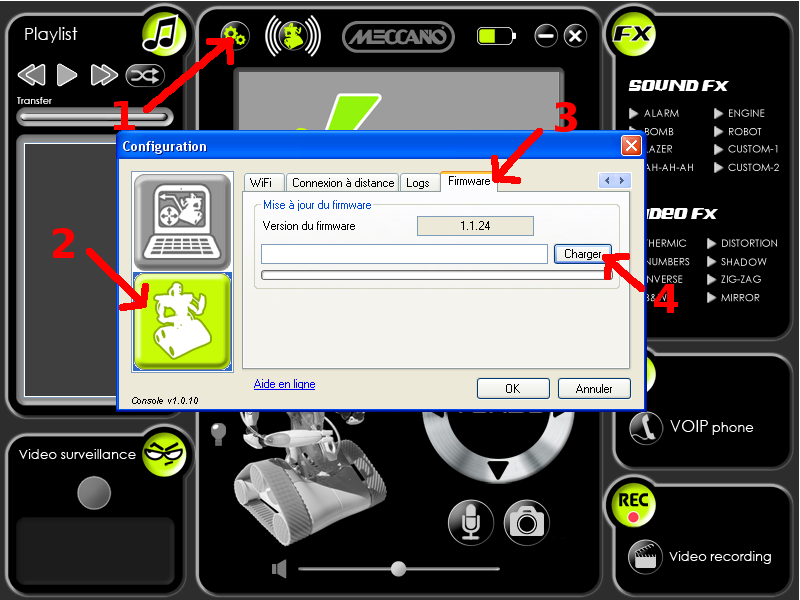
\includegraphics[width=0.95\textwidth]{img/spykee-flash-instructions}
\end{center}

With the Urbi firmware, the Spykee should continue to work as usual: you can
still control it using the Spykee interface. But you can now also control it
with Urbi. Please read the Urbi tutorial if you do not know how to communicate
with an urbi server.

\section{Device list}

The following standard devices are available on the Spykee:

\begin{itemize}
\item \lstinline|trackL, trackR (Motor)| \\
    The two tracks. The \lstinline|val| slot can be read or set to change each
    track speed, from -100 to 100.
\item \lstinline|ledL, ledR, flash (Led)| \\
    left and rigth led pairs, and camera light. On if the \lstinline|val| slot
    is set to 1.
\item \lstinline|camera (VideoIn)| \\
    Spykee camera. The \lstinline|val| slot contains the last received image
    in jpeg format.
\item \lstinline|speaker (AudioOut)| \\
    Sound speaker.
\item \lstinline|micro (AudioIn)| \\
    Microphone.
\item \lstinline|robot (Mobile)| \\
    Provides the standard functions go() and turn().
\end{itemize}

The following non-standard functions are also present:

\begin{itemize}
\item \lstinline|speaker.playSound(id)| \\
    Play Spykee sound sample "id", from 0 to 15.
\item \lstinline|mp3.play(stream)| \\
    Play mp3 file or http stream "stream".
\item \lstinline|mp3.stop()| \\
    Stop playing current stream or file.
\item \lstinline|Spykee.setConfigValue(key, value)| \\
    Set persistant config entry "key" to "value". Beware that the configuration
    sector only have a few kilobytes of space, do not put too many or to big
    values here.
\item \lstinline|Spykee.getConfigValue(key)| \\
    Retrieve persistant value associated with "key". Do not call this function
    two often as it is very costly.
\item \lstinline|Spykee.findBase()| \\
    Ask the Spykee to look for its base and station on it.
\item \lstinline|Spykee.cancelFindBase()| \\
    Abort the previous order.
\item \lstinline|Spykee.chargeStop()| \\
    Ask the Spykee to stop charging and exit its charging station.
\item \lstinline|Spykee.power| \\
    Remaining energy in the battery, from 0 to 100. The value may be inaccurate
    or outside the range while the Spykee is charging.
\end{itemize}

\section{Dynamically loaded modules}
At startuup, the Spykee tries to connect to the spykee.gostai.com website to
fetch a list of additional features available for download.
It sets up the system in a way that the first attempt to use one of those
additional features will download and load the required objects.

The location where the modules are fetched can be changed by setting the
\lstinline|loader_host| and \lstinline|loader_dir| config values (using
\lstinline|Spykee.setConfigValue()|).
Default values are \em{spykee.gostai.com} and \em{/modules/}.

The following modules are currently available:

\subsection{Clapper}

The Clapper module detects and counts short and loud sounds, such as the one
made by clapping one's hands. It can be instanciated by typing:

\begin{urbiunchecked}
var Global.clap = Clapper.new("micro.val", 0.2, 200, 800, 4000);
\end{urbiunchecked}

The second parameter is the volume threshold above which a clap is detected.
The third and fourth parameters are the minimum and maximum delay between claps,
in milliseconds. The last argument is the maximum duration of a sound sequence.

Each time a clap sequence ends, the \lstinline|val| slot of the object is
set to the number of claps heard, then reset to 0.
Additionnaly, if \lstinline|emitEvent| is true, the event \lstinline|sequence|
is emited with one argument: the number of claps heard.

\begin{urbiunchecked}
clap.emitEvent = 1;
// Play sound sample number 3 when two successive claps are heard.
tag:at(clap.sequence?(2)) speaker.playSound(3);
// Stop the previous behavior.
tag.stop;
\end{urbiunchecked}
